%%%%%%%%%%%%%%%%%%%%%%%%%%%%%%%%%%%%%%%%%%%%%%%%%%%%%%%%%%%%%%%%%%%%%%%%
\clearpage
\section{Plugin functions for SESANS}
\label{ch:pluginsSESANS}

An overview about the transformation cycle between the spherically symmetric correlation function, projected correlation function and differential cross section, which is relevant for the SESANS plugin functions, is described in detail in \cite{Kohlbrecher2017}.

The depolarization of the neutron beam as a function of the spin-echo length $z$ is given by
\begin{align}
\frac{P_n(\delta)}{P_{n0}(\delta)}&=\exp\left(\mathcal{G}(\delta)-\mathcal{G}(0)\right)
\end{align}
where the unnormalized SESANS correlation function reads as
\begin{align}
\mathcal{G}(\delta) &= \frac{1}{k_0^2} \int_{-\infty}^{\infty}\int_{-\infty}^{\infty} \mathrm{d}Q_y\, \mathrm{d}Q_z \frac{\mathrm{d}\Sigma(\mathbf{Q})}{\mathrm{d}\Omega}\frac{\cos(Q_z \delta)}{S} \\
             &= \frac{1}{k_0^2} \int_{-\infty}^{\infty}\int_{-\infty}^{\infty} \mathrm{d}Q_y\, \mathrm{d}Q_z  \frac{\mathrm{d}\sigma(\mathbf{Q})}{\mathrm{d}\Omega}t \cos(Q_z \delta)
\end{align}
with $\mathbf{Q}=(0,Q_y,Q_z)^T$ and $\frac{\mathrm{d}\Sigma(\mathbf{Q})}{\mathrm{d}\Omega}$ being the macroscopic differential scattering cross-section in units of cm$^2$ and $\frac{\mathrm{d}\sigma(\mathbf{Q})}{\mathrm{d}\Omega}=\frac{1}{V}\frac{\mathrm{d}\Sigma(\mathbf{Q})}{\mathrm{d}\Omega}$ the differential scattering cross-section normalized on the sample volume $V=tS$ in units of cm$^{-1}$. $t$ is the sample thickness and $S$ the aperture cross-section defining the illuminated sample area. For isotropic scattering $\frac{\mathrm{d}\sigma(\mathbf{Q})}{\mathrm{d}\Omega}=\frac{\mathrm{d}\sigma(Q)}{\mathrm{d}\Omega}$, where the scattering only depends on the modulus of the scattering vector $Q=\abs{\mathbf{Q}}$ the unnormalized SESANS correlation function simplifies to a Hankel transform of the scattering intensity multiplied by $\frac{\lambda^2 t}{2\pi}$. To see this, one has to change from cartesian coordinates $(0,Q_y,Q_z)$ to polar coordinates $Q (0,\sin\phi,\cos\phi)$ with $\mathrm{d}Q_y \mathrm{d}Q_z = Q\mathrm{d}Q \mathrm{d}\phi$. The integration over $\phi$ yield the cylindrical zeroth-order Bessel function
\begin{align}
J_0(Qz)=\frac{1}{2\pi}\int_{0}^{2\pi} \cos\left(Q\cos(\phi)\delta\right) \mathrm{d}\phi
\end{align}
so that one gets
\begin{align}
\mathcal{G}(\delta) &= \frac{2\pi t}{k_0^2} \int_{0}^{\infty} Q J_0(Q\delta) \frac{\mathrm{d}\sigma(Q)}{\mathrm{d}\Omega} \, \mathrm{d}Q \\
&= \frac{\lambda^2 t}{4\pi^2} 2\pi\underbrace{\int_{0}^{\infty} Q J_0(Q\delta) \frac{\mathrm{d}\sigma(Q)}{\mathrm{d}\Omega} \, \mathrm{d}Q}_{\mathcal{H}_0\left[\frac{\mathrm{d}\sigma(Q)}{\mathrm{d}\Omega}\right](\delta)} = \frac{\lambda^2 t}{4\pi^2}  2\pi \mathcal{H}_0\left[\frac{\mathrm{d}\sigma(Q)}{\mathrm{d}\Omega}\right](\delta)
= \lambda^2 t \tilde{G}(\delta)
\end{align}
where $\tilde{G}(\delta)=\frac{1}{2\pi}\mathcal{H}_0\left[\frac{\mathrm{d}\sigma(Q)}{\mathrm{d}\Omega}\right](\delta)$. $\mathcal{H}_0\left[\ldots\right]$ denotes the Hankel transform of zeroth order.\footnote{\label{footnote:Hankel}
There are several possible definitions of a Hankel transform $\mathcal{H}_\nu\left[f(r)\right]$ of order $\nu$ of a function $f(r)$ and its inverse $\mathcal{H}_\nu^{-1}\left[F_\nu(k)\right]$
\begin{enumerate}
\item $F_\nu(k) = \int_0^\infty f(r) J_\nu(kr) r \,\mathrm{d}r$ and its inverse $f(r)=\int_0^\infty F_\nu(k)J_\nu(kr) k \,\mathrm{d}k$
\item $F_\nu(k) = \int_0^\infty f(r) J_\nu(kr) \sqrt{kr} \,\mathrm{d}r$ and its inverse $f(r)=\int_0^\infty F_\nu(k)J_\nu(kr)  \sqrt{kr}  \, \mathrm{d}k$
\item $F_\nu(k) = 2\pi \int_0^\infty f(r) J_\nu(2\pi kr) r \,\mathrm{d}r$ and its inverse $f(r)=2\pi \int_0^\infty F_\nu(q)J_\nu(2\pi kr) k \,\mathrm{d}k$
\end{enumerate}
}
Experimentally the differential cross-section is only measured up to a maximum scattering angle $\Theta_\mathrm{max}$. Because of this \SASfit supplies is clipping the Hankel transform of the model of the differential cross-section if the experimental data supplied with a fourth column containing the maximum scattering vector for each spin echo length $Q_\mathrm{max}=\frac{4\pi}{\lambda}\sin \Theta_\mathrm{max}/2$. This clipping is activated by activating the resolution option.

The instrument independent projected sample correlation function $\tilde{G}(\delta)$ can also be calculated via the Abel transform $\mathcal{A}$ of the scattering length density autocorrelation function $\tilde{\gamma}(\mathbf{r})=\int \rho(\mathbf{r'})\rho(\mathbf{r'-r})\mathrm{d}\mathbf{r'}$.
\begin{align}
\tilde{G}(\delta) &= 2 \int_z^\infty \frac{\tilde{\gamma}(r) r}{\sqrt{r^2-z^2}} \mathrm{d}r = \mathcal{A}\left[\tilde{\gamma}(r)\right](\delta)
\end{align}
The scattering intensity $I(Q)$ and  $\tilde{\gamma}(r)$ are related by Fourier transform\footnote{\label{footnote:Fourier}Similar to the Hankel transform also for the Fourier transform several conventions (spherical symmetric functions are assumed here) are in use which are
\begin{enumerate}
\item $\mathcal{F}_{I,3D}[f(r)](Q)=F(Q)=\int_0^\infty f(r) \frac{\sin 2\pi Qr}{2\pi Qr}4\pi r^2\mathrm{d}r$ and \\ $\mathcal{F}_{I,3D}^{-1}[F(Q)](r)=f(r)=\int_0^\infty F(Q) \frac{\sin 2\pi Qr}{2\pi Qr}4\pi r^2\mathrm{d}Q$
\item $\mathcal{F}_{I,3D}[f(r)](Q)=F(Q)=\int_0^\infty f(r) \frac{\sin Qr}{Qr}4\pi r^2\mathrm{d}r$ and \\ $\mathcal{F}_{I,3D}^{-1}[F(Q)](r)=f(r)=\frac{1}{(2\pi)^3}\int_0^\infty F(Q) \frac{\sin Qr}{Qr}4\pi r^2\mathrm{d}Q$
\item $\mathcal{F}_{I,3D}[f(r)](Q)=F(Q)=\frac{1}{(2\pi)^{3/2}}\int_0^\infty f(r) \frac{\sin Qr}{ Qr}4\pi r^2\mathrm{d}r$ and \\ $\mathcal{F}_{I,3D}^{-1}[F(Q)](r)=f(r)=\frac{1}{(2\pi)^{3/2}}\int_0^\infty F(Q) \frac{\sin Qr}{Qr}4\pi r^2\mathrm{d}Q$
\end{enumerate}
In small angle scattering convention 2 is normally used.
} $\mathcal{F}_{I,3D}[\ldots]$
\begin{align}
I(Q) &= \int_0^\infty \tilde{\gamma}(r) \frac{\sin Qr}{Qr}4\pi r^2\mathrm{d}r =
\mathcal{F}_{I,3D}\left[\tilde{\gamma}(r)\right](Q)
\end{align}
In literature the expressions for the scattering length density autocorrelation function are often normalized to to 1 for $r=0$, i.e. the expressions $\gamma_0(r)=\tilde{\gamma}(r)/\tilde{\gamma}(0)$ are given. Also one finds that
\begin{align}
\tilde{\gamma}(0)&=\Delta\eta^2 V_P
\end{align}
and
\begin{align}
\int_0^\infty \tilde{\gamma}(r) 4\pi r^2 \, \mathrm{d}r =\Delta\eta^2 V_P^2 \quad \mbox{or} \quad  \int_0^\infty \gamma_0(r) 4\pi r^2 \, \mathrm{d}r = V_P
\end{align}
where in case of spherical particle $V_P=\frac43 \pi R^3$
In Fig.\ \ref{fig:FAHcycle} it is shown how the functions $\tilde{\gamma}(r)$, $\tilde{G}(\delta)$ and $IQ)$ are related to each other. However, the cycle is mathematically only exact for a one-dimensional Fourier transformation on a radial symmetric function. Such a transformation cycle is called the projection-slice theorem which is a standard analysis in imaging \cite{Bracewell2003, Bracewell1956}. The projection-slice theorem makes use of the fact that
\begin{align}
\mathcal{H}\circ \mathcal{F}_{1D}\circ \mathcal{A} &
              =\mathcal{F}_{1D} \circ \mathcal{A}\circ \mathcal{H}
              =\mathcal{A}\circ \mathcal{H}\circ \mathcal{F}_{1D}=\mathcal{I}
\end{align}
with $\mathcal{F}_{1D}(s)=\int_{-\infty}^{\infty} \exp\left(-\imath 2\pi s r\right) f(r) \mathrm{d}r$, i.e. using the pair (1) of Fourier as well pair (1) of Hankel transform conventions as given in footnote\footref{footnote:Fourier} and footnote\footref{footnote:Hankel}.
That the $\mathcal{FAH}$ cycle is still valid using the isotropic 3 dimensional Fourier transform $\mathcal{F}_{I,3D}$ as shown in fig.\ \ref{fig:FAHcycle} has been shown in \cite{Kohlbrecher2017}.

\begin{figure}[htb]
\begin{center}
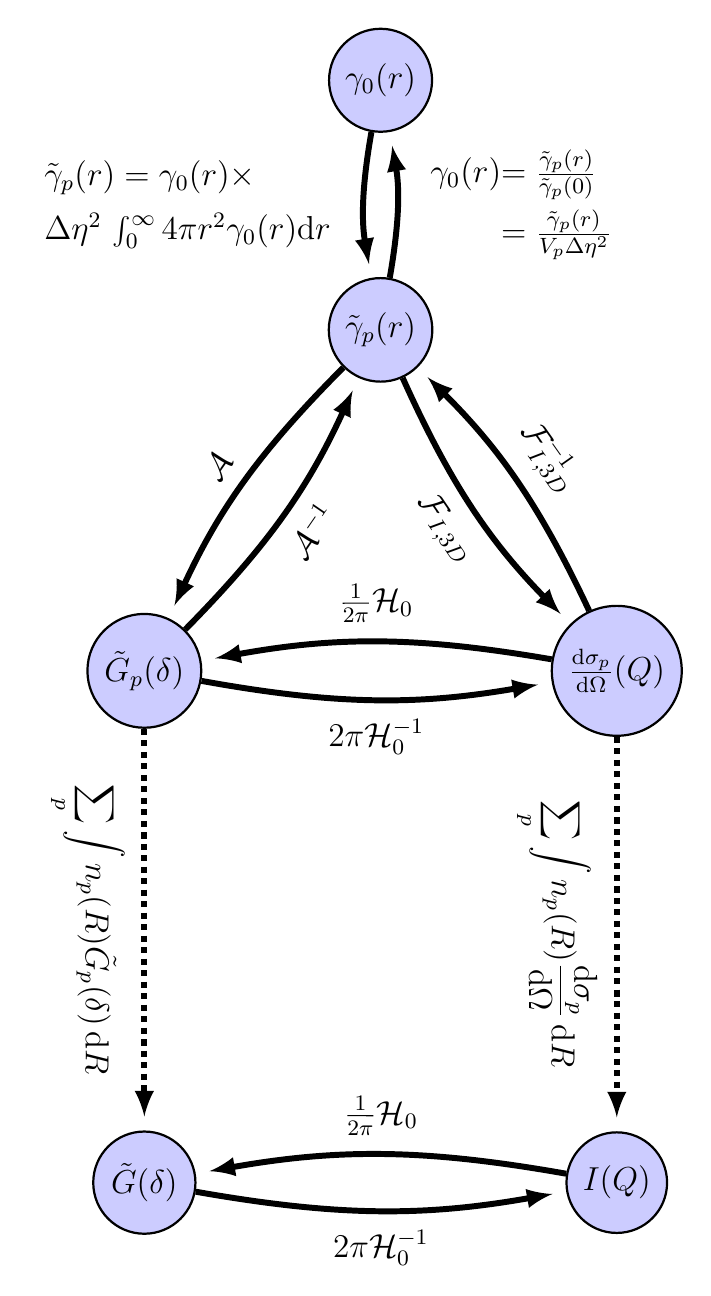
\begin{tikzpicture}[->,>=stealth,shorten >=5pt,auto,node distance=1cm,
  thick,main node/.style={circle,fill=blue!20,draw,
  font=\sffamily\large\bfseries,minimum size=10mm}]

  \node[main node] (gamma0) at (3,7.5) {$\gamma_0(r)$};
  \node[main node] (gamma) at (3,4.33) {$\tilde{\gamma}_p(r)$};
  \node[main node] (IQp) at (6,0) {$\frac{\mathrm{d}\sigma_p}{\mathrm{d}\Omega}(Q)$};
  \node[main node] (Gp) at (0,0) {$\tilde{G}_p(\delta)$};
  \node[main node] (Gz) at (0,-6.5) {$\tilde{G}(\delta)$};
  \node[main node] (IQ) at (6,-6.5) {$I(Q)$};
   \pgfsetarrowsend{latex}
  \pgfsetlinewidth{0.5ex}
  \path[every node/.style={font=\sffamily\large,
  		fill=white,inner sep=1pt}]
  	% Right-hand-side arrows rendered from top to bottom to
  	% achieve proper rendering of labels over arrows.

    (gamma0) edge [bend right=10] node[outer sep=6pt,pos=0.5,left] {
    $\begin{array}{l}
       \tilde{\gamma}_p(r) = \gamma_0(r) \times\\[2mm]
       \Delta\eta^2\, \int_0^\infty 4\pi r^2 \gamma_0(r) \mathrm{d}r
     \end{array}$} (gamma)
    (gamma) edge [bend right=10] node[outer sep=6pt,pos=0.5,right] { $ \begin{array}{ll} \gamma_0(r)\!\!\!\!\! &= \frac{\tilde{\gamma}_p(r)}{\tilde{\gamma}_p(0)}\\[2mm] &=\frac{\tilde{\gamma}_p(r)}{V_p\Delta\eta^2}\end{array}$} (gamma0)
    (gamma) edge [bend right=10] node[outer sep=6pt,pos=0.5,sloped,below] { $ \mathcal{F}_{I,3D}$} (IQp)
            edge [bend right=10] node[outer sep=6pt,pos=0.5,sloped,above] { $ \mathcal{A}$} (Gp)
    (Gp) edge [bend right=10] node[outer sep=6pt,pos=0.5,sloped,below] { $ {2\pi}\mathcal{H}_0^{-1}$} (IQp)
         edge [bend right=10] node[outer sep=6pt,pos=0.5,sloped,below] { $ \mathcal{A}^{-1}$} (gamma)
         edge [bend right=0,dotted] node[outer sep=6pt,pos=0.5,sloped,below] {  $ \displaystyle \sum_p \int n_p(R) \tilde{G}_p(\delta)\, \mathrm{d}R$} (Gz)
    (IQp) edge [bend right=10] node[outer sep=6pt,pos=0.5,sloped,above] { $ \frac{1}{2\pi}\mathcal{H}_0$} (Gp)
         edge [bend right=10] node[outer sep=6pt,pos=0.5,sloped,above] { $ \mathcal{F}_{I,3D}^{-1}$} (gamma)
         edge [bend right=0,dotted] node[outer sep=6pt,pos=0.5,sloped,below] { $ \displaystyle \sum_p\int n_p(R)\frac{\mathrm{d}\sigma_p}{\mathrm{d}\Omega}\, \mathrm{d}R$} (IQ)
    (IQ) edge [bend right=10] node[outer sep=6pt,pos=0.5,sloped,above] { $ \frac{1}{2\pi}\mathcal{H}_0$} (Gz)
    (Gz) edge [bend right=10] node[outer sep=6pt,pos=0.5,sloped,below] { $ {2\pi}\mathcal{H}_0^{-1}$} (IQ);
\end{tikzpicture}
\end{center}
\caption{Transformation cycle between $\tilde{\gamma}(r)$, $I(q)$, and $\tilde{G}(\delta)$.}\label{fig:FAHcycle}
\end{figure}

\begin{figure}[htb]
\begin{center}
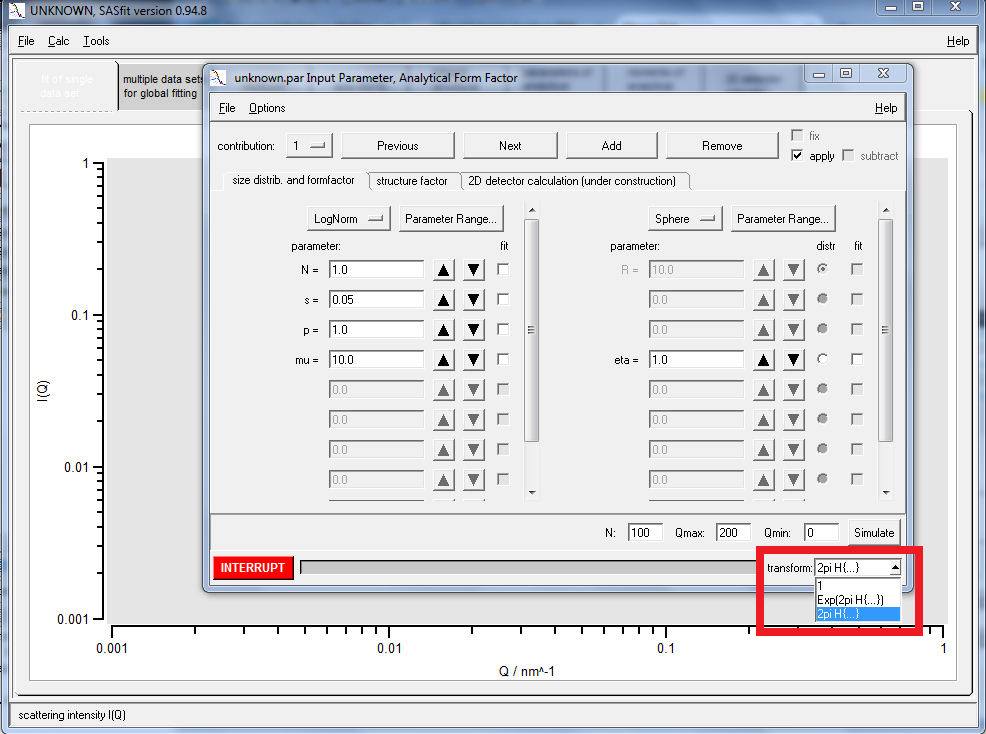
\includegraphics[width=0.7\textwidth]{../images/GUI/HankelOperator.png}
\end{center}
\caption{\SASfit allows to perform a final transformation on the model function to convert a SANS signal into a SESANS signal}
\label{fig:HankelOp}
\end{figure}


\subsection{$G(\delta)$ of a sphere} ~\\
\label{sec:Gz_sphere}
The scattering intensity for a single sphere is given by
\begin{align}
I(Q) &= \left(\frac{4}{3}\pi R^3 \Delta\eta\right)^2 \left(3\frac{\sin QR-QR\cos QR}{Q^3R^3}\right)^2
\end{align}
The unnormalized autocorrelation function for this sphere is given by
\begin{align}
\tilde{\gamma}(r) &=
\begin{cases}
 \Delta\eta^2  \frac{4}{3}\pi R^3 \left( 1-\frac{3}{4}\frac{r}{R}+\frac{1}{16}\left(\frac{r}{R}\right)^3\right) & \mbox{for } r\leq 2R \\
0 & \mbox{for }  r>2R
\end{cases}
\end{align}
and the unnormalized SESANS correlation function
\begin{align}
\begin{split}
\tilde{G}_\mathrm{sph}(\delta)&= \Delta\eta^2 \pi R^4 \\
&\times \left(\sqrt{1-\xi^2}(2+\xi^2)-\xi^2(\xi^2-4)\ln\left(\frac{\xi}{1+\sqrt{1-\xi^2}}\right)\right)
\end{split}
\label{eq:Gz_sph}
\end{align}
with $\xi=\frac{\delta}{2R}$.


\hspace{1pt}\\
\underline{Input Parameters for model \texttt{G\_Sphere(delta)}:}\\
\begin{description}
\item[\texttt{R}] radius of sphere $R$
\item[\texttt{dummy}] not used
\item[\texttt{dummy}] not used
\item[\texttt{eta}] scattering length density contrast $\Delta\eta$
\end{description}

\hspace{1pt}\\
\underline{Note:}
\begin{itemize}
\item the function \texttt{G\_Sphere(delta)} can be combined with a size distribution but should not be combined with a structure factor.
\end{itemize}

\begin{figure}[htb]
\begin{center}
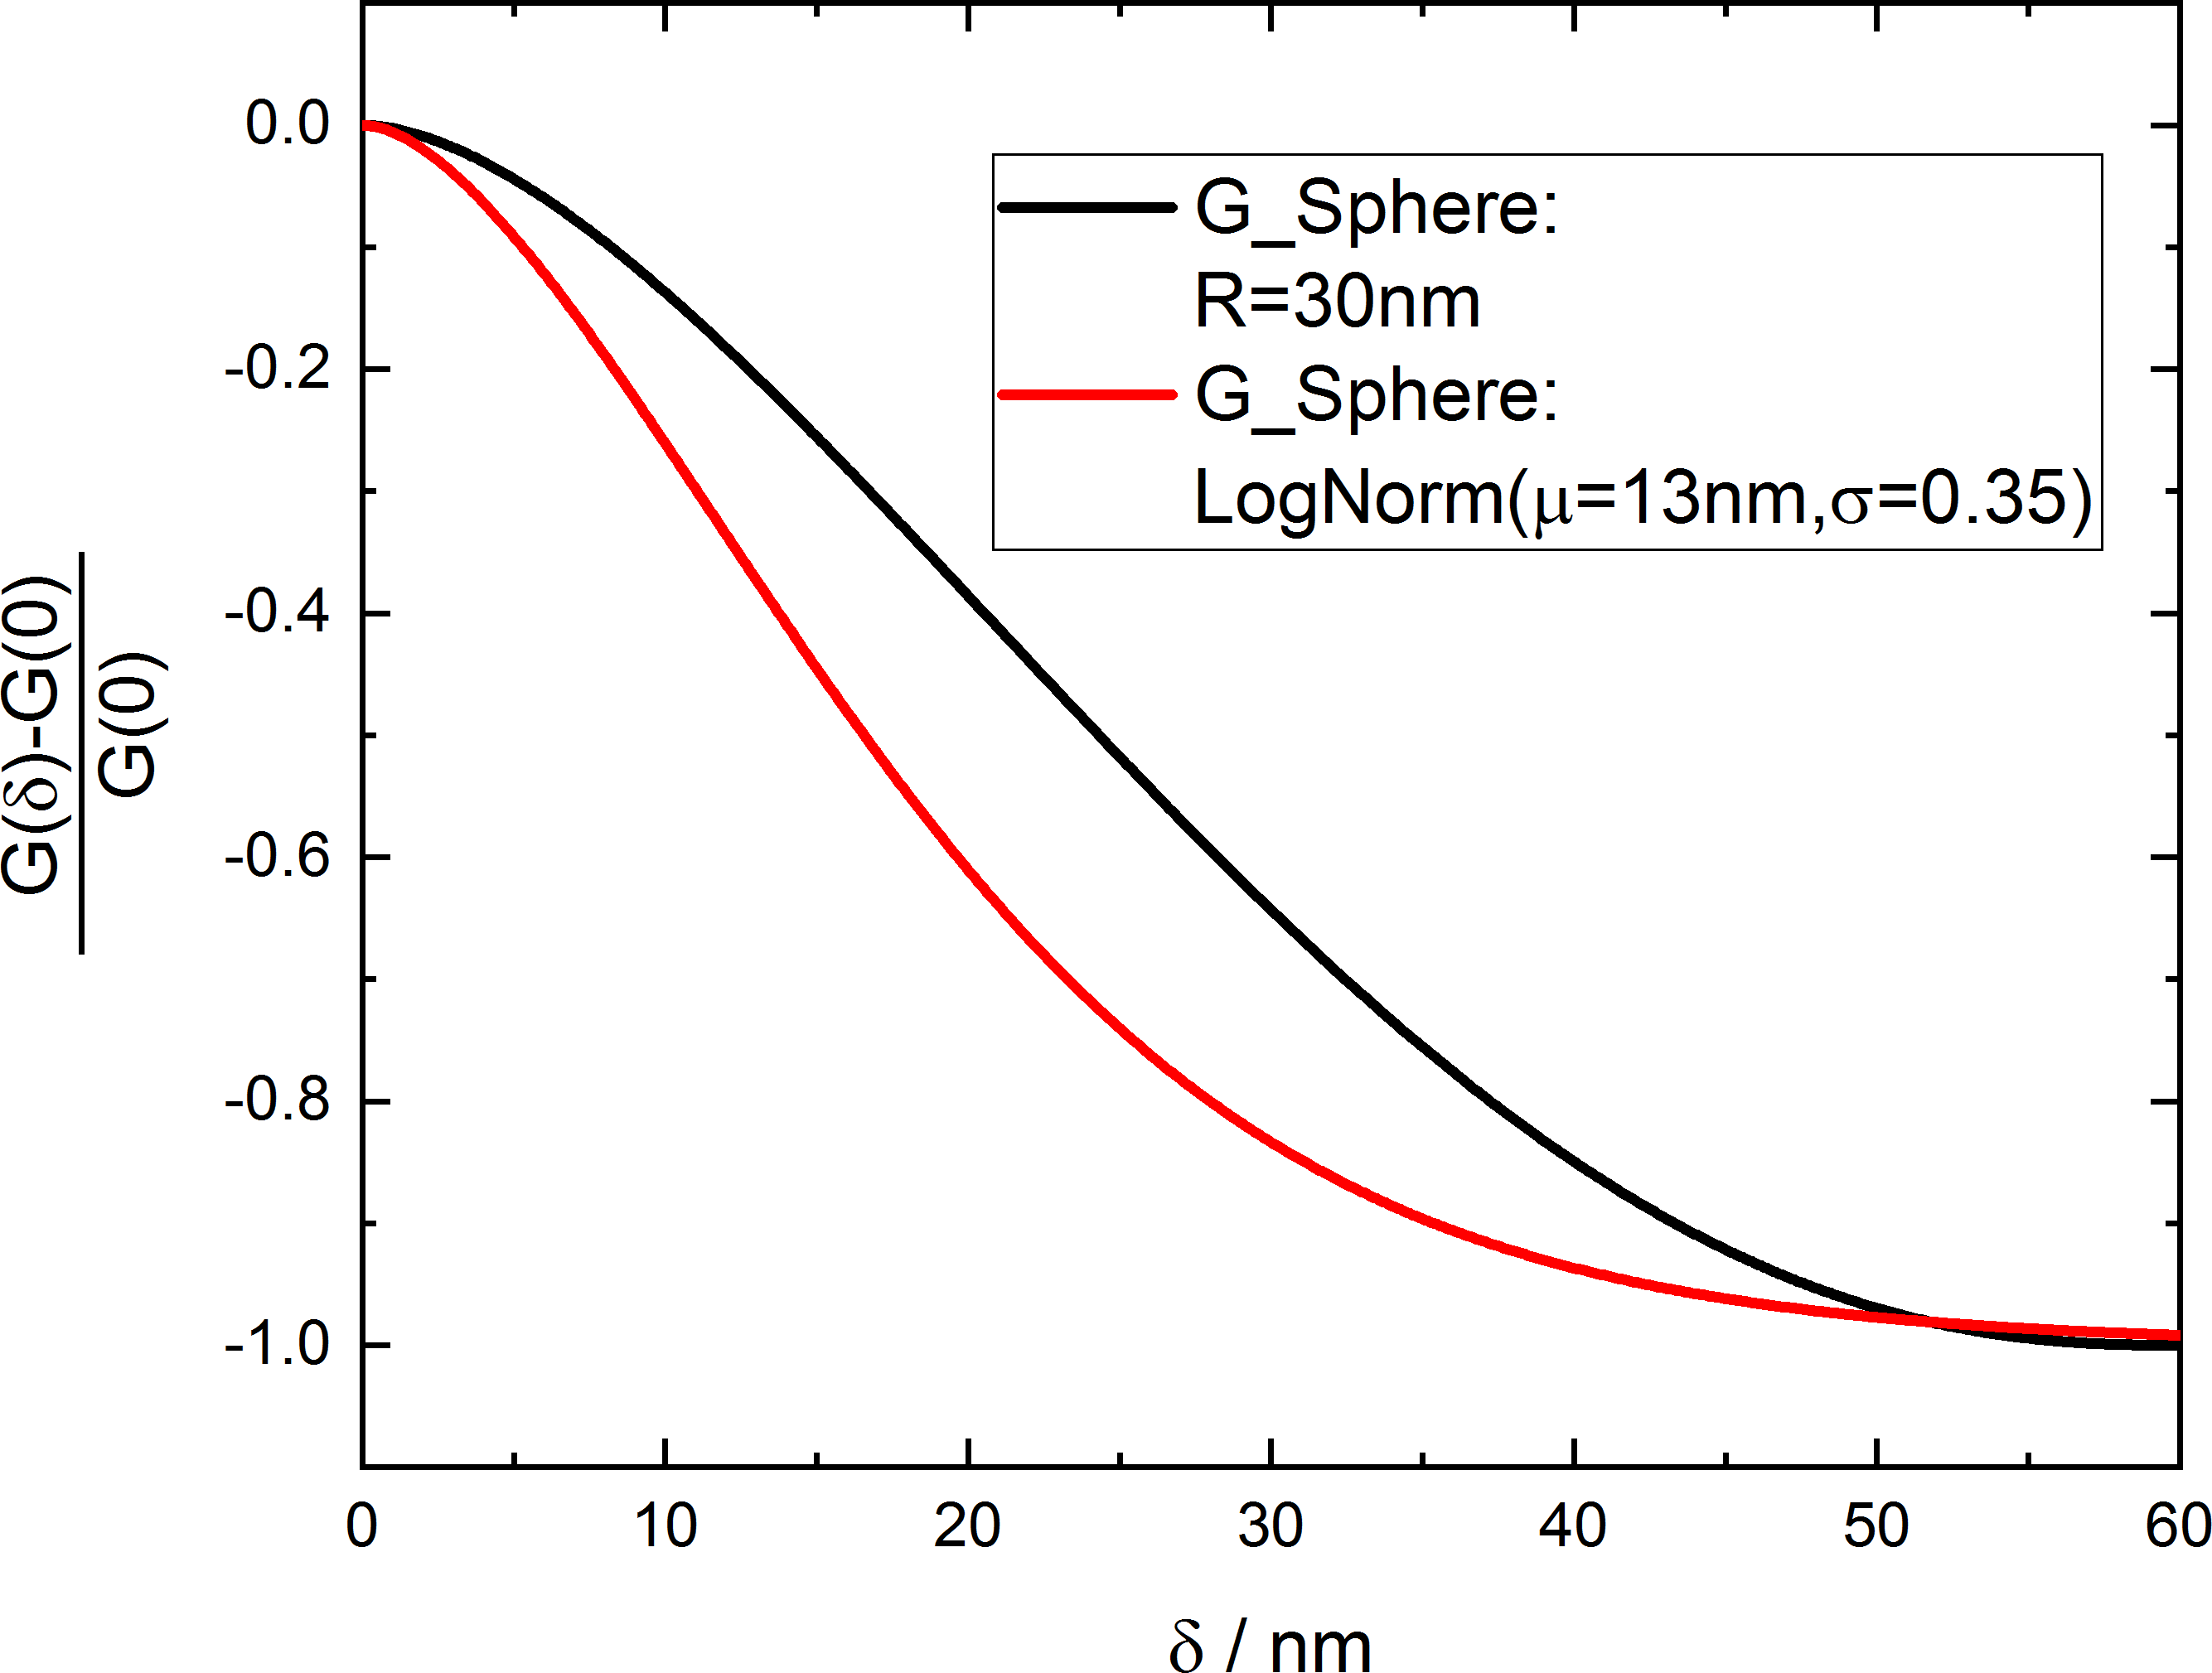
\includegraphics[width=0.7\textwidth]{../images/form_factor/SESANS/G_Sphere.png}
\end{center}
\caption{Projected correlation functions of monodisperse spheres and polydisperse Spheres, both with a $R_g=24.5$nm}
\label{fig:G_Sphere}
\end{figure}

\subsection{$G(\delta)$ of a randomly distributed, two-phase system (DAB) and its generalisation (gDAB)}~\\
\label{sec:Gz_DAB_gDAB}

The scattering intensity for a randomly distributed, two-phase system (DAB) is given by
\cite{DebyeBueche1949,DAB1957,Andersson2008}
\begin{align}
I(Q) &= \frac{\left(8 \pi \xi^3 \Delta\eta\right)^2}{ \left(1+Q^2\xi^2\right)^2}
\end{align}
The unnormalized autocorrelation function for the two-phase system reads as
\begin{align}
\tilde{\gamma}(r) &=
 \Delta\eta^2 8\pi\xi^3 \exp\left( -r/\xi\right)
\end{align}
and the unnormalized SESANS correlation function as
\begin{align}
\tilde{G}_\mathrm{DAB}(\delta)&= 8\pi\xi^4 2\frac{\delta}{\xi}K_1\left(\frac{\delta}{\xi}\right)
\end{align}

The scattering intensity for a randomly distributed, self-affine two-phase system (gDAB) is given by \cite{Klimes2002,Hunter2006,Andersson2008}
\begin{align}
I(Q) &= \frac{V_P^2\Delta\eta^2}{\left[1+(q\xi)^2\right]^{\frac32+H}}
\end{align}
The unnormalized autocorrelation function for this system is given by
\begin{align}
\tilde{\gamma}(r) &= \Delta\eta^2 V_P \gamma_0(r) \\
                  &= \Delta\eta^2 V_P \frac{2}{\Gamma(H)}\left(\frac{r}{2\xi}\right)^H K_H\left(\frac{r}{\xi}\right) \\
 V_P &= \left(2\xi\sqrt{\pi}\right)^3\frac{\Gamma\left(\frac{3}{2}+H\right)}{\Gamma\left(H\right)}
\end{align}
and the unnormalised SESANS correlation function
\begin{align}
\tilde{G}_\mathrm{gDAB}(\delta)&=  
\frac{\Delta\eta^2V_P^2}{2\pi\xi^2\Gamma\left(\frac32+H\right)}\left(\frac{\delta}{2\xi}\right)^{\frac12+H}K_{\frac12+H}\left(\frac{\delta}{\xi}\right)
%8\xi^3\pi\sqrt{\pi}\frac{\Gamma\left(\frac{3}{2}+H\right)}{\Gamma^2\left(H\right)}
% 2\sqrt{\xi\delta}\left(\frac{\delta}{2\xi}\right)^{H+\frac12}K_{\frac12+H}\left(\frac{\delta}{\xi}\right)
\label{eq:Gz_gDAB}
\end{align}

\hspace{1pt}\\
\underline{Input Parameters for model \texttt{G\_DAB(delta)}}:}\\
\begin{description}
\item[\texttt{xi}] correlation length $\xi$
\item[\texttt{dummy}] not used
\item[\texttt{dummy}] not used
\item[\texttt{eta}] scattering length density contrast $\Delta\eta$
\end{description}

\hspace{1pt}\\
\underline{Input Parameters for model \texttt{G\_gDAB(delta)}:}\\
\begin{description}
\item[\texttt{xi}] correlation length $\xi$
\item[\texttt{H}] Hurst exponent
\item[\texttt{dummy}] not used
\item[\texttt{eta}] scattering length density contrast $\Delta\eta$
\end{description}

\hspace{1pt}\\
\underline{Note:}
\begin{itemize}
\item the Hurst exponent needs to be in the interval $H \in (0,1]$. Values of $H>1$ as well as $H\in(-\frac12,0]$ will be accepted but might not have an established interpretation.
\item the functions \texttt{G\_DAB(delta)} and \texttt{G\_gDAB(delta)}can be combined with a size distribution but should not be combined with a structure factor.
\end{itemize}

\begin{figure}[htb]
\begin{center}
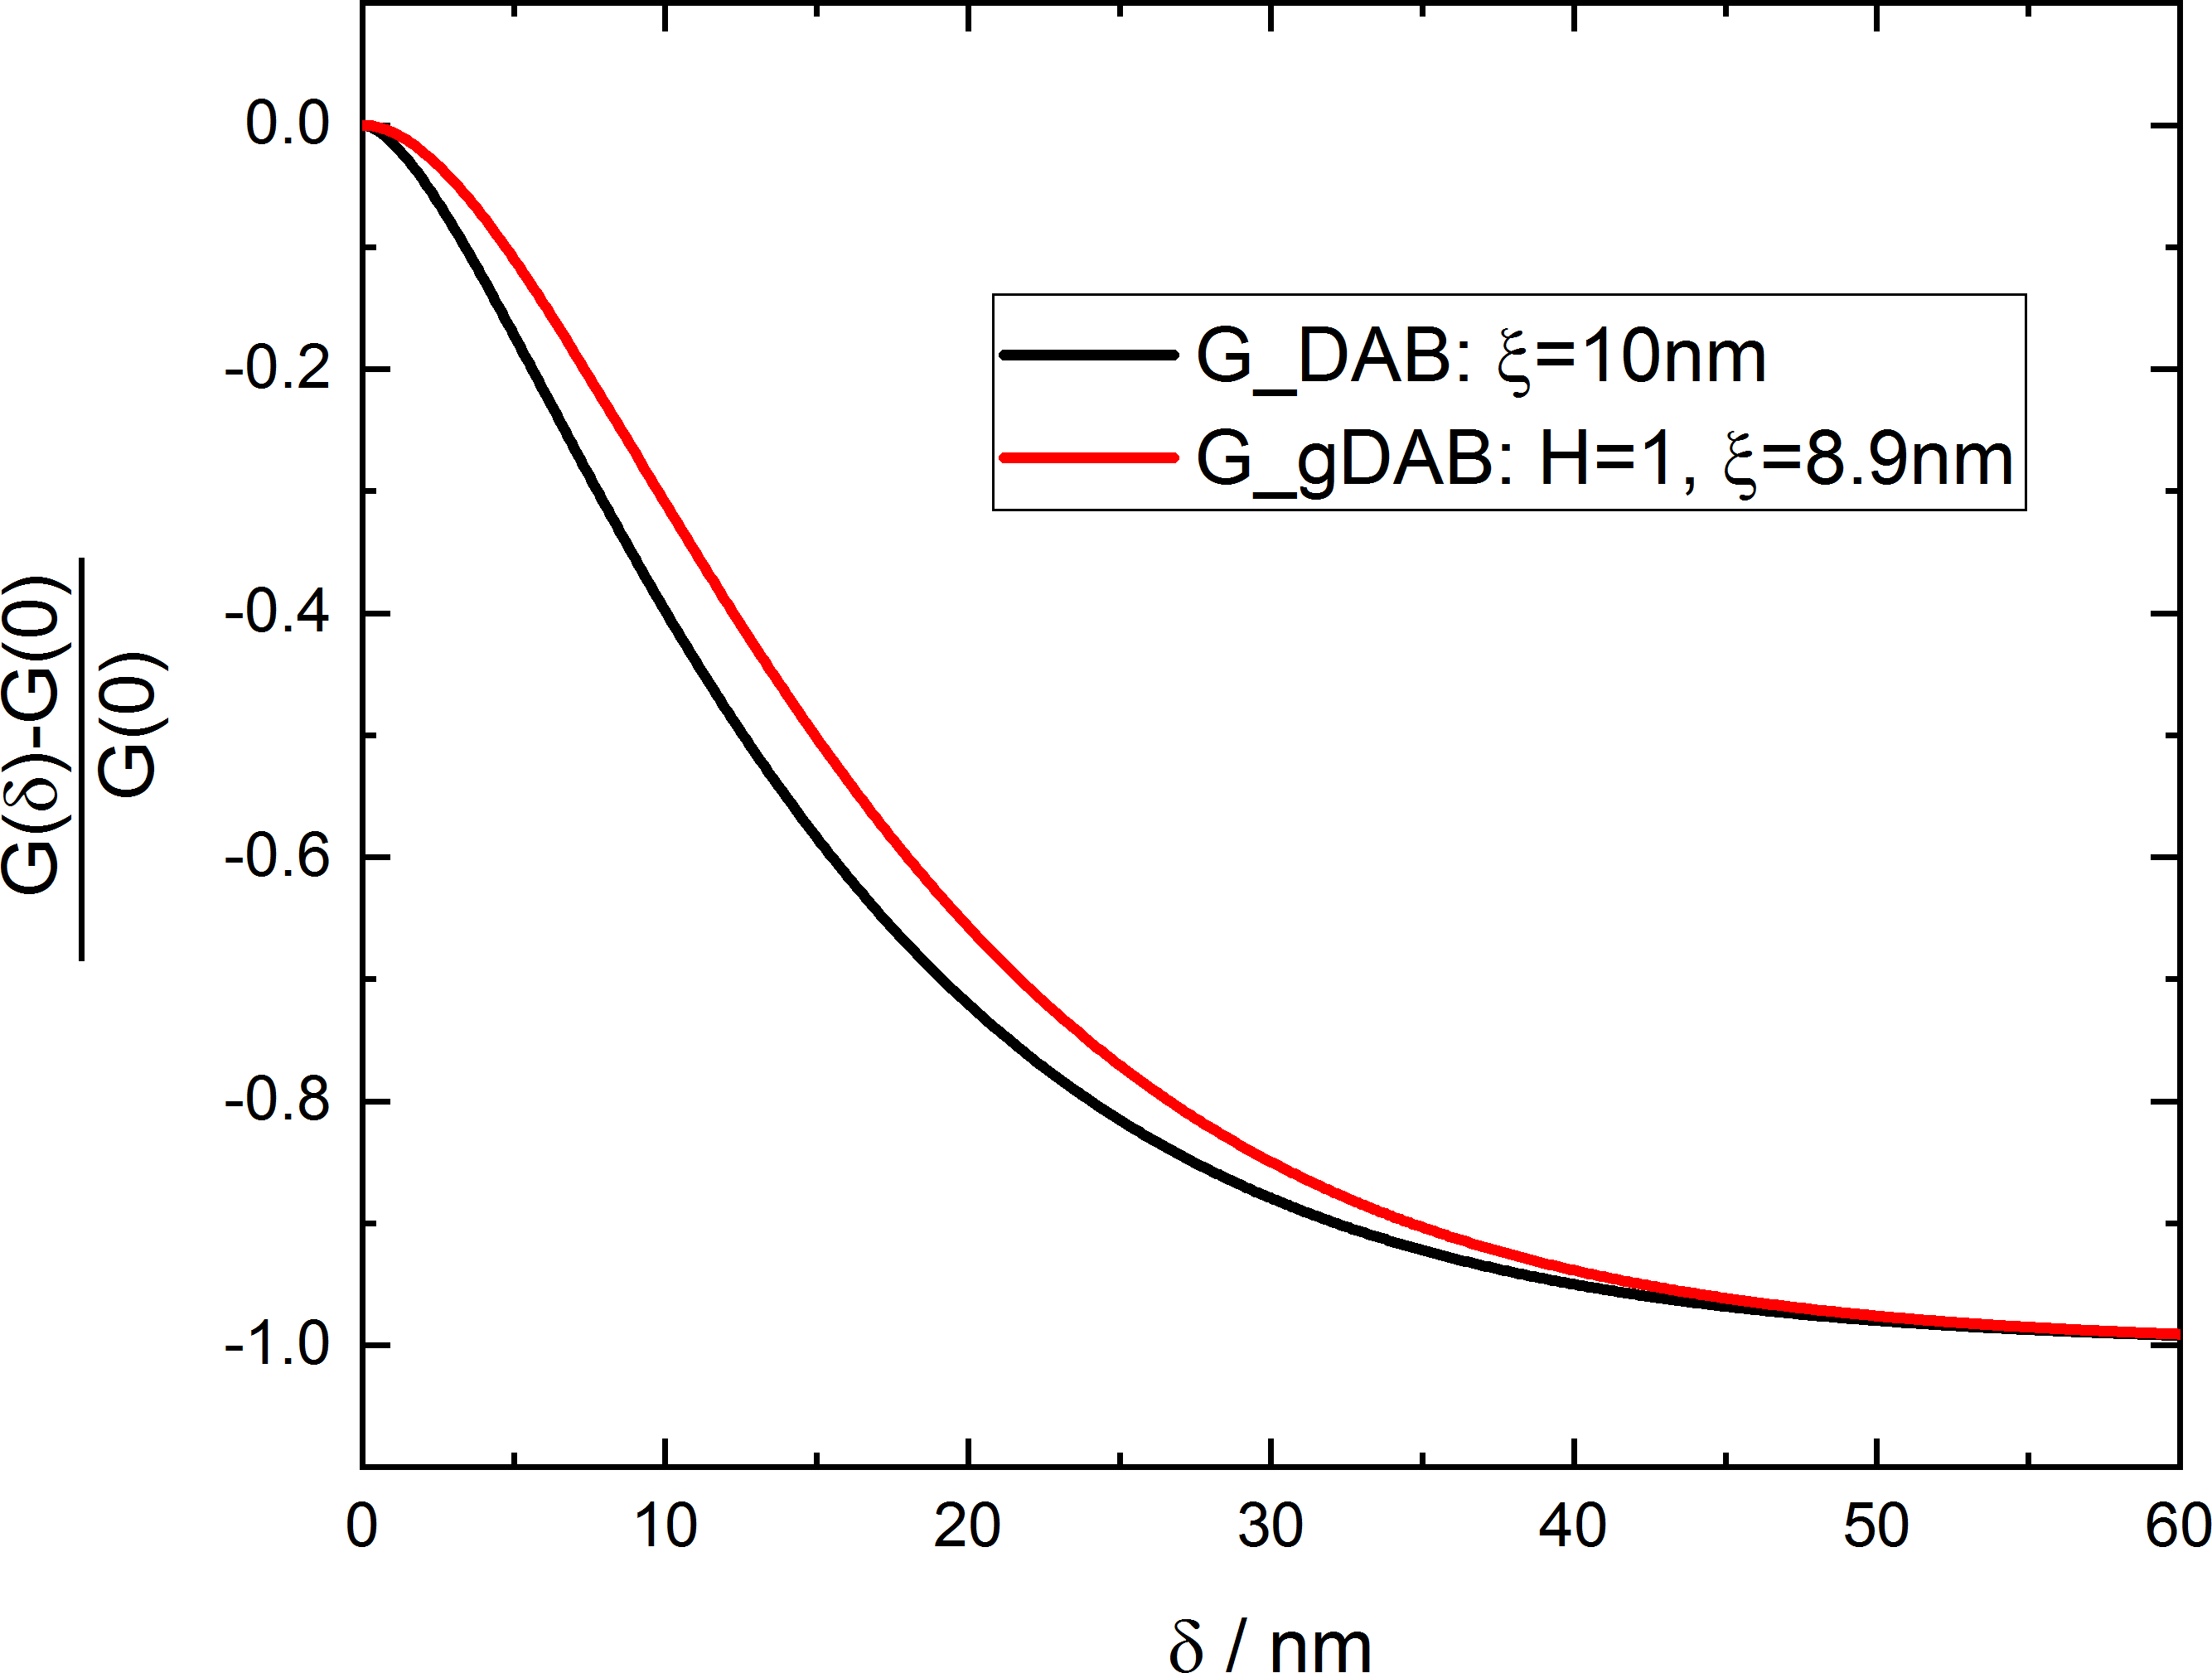
\includegraphics[width=0.7\textwidth]{../images/form_factor/SESANS/G_gDAB.png}
\end{center}
\caption{Projected correlation functions of the Debye-Andersson-Brumberger model and its generalisation with an Hurst exponent of $H=1$ but both with a $R_g=24.5nm$}
\label{fig:G_gDAB}
\end{figure}


\subsection{$G(\delta)$ for a generalized Gaussian coil (gGc) }~\\
\label{sec:Gz_gGc}
The scattering intensity for a a generalized Gaussian coil (gGc) has been given by  Hammouda \cite{Hammouda,Hammouda2012,Hammouda1993,Hammouda2016} (see also section \ref{sect:generalized_gaussian_coil}) as
\begin{align}
I_\text{gGc}(q) &= I_0
\left(
\frac{1}{\nu U^{\frac{1}{2 \nu}}} \; \gamma\left(\frac{1}{2 \nu},U\right)-
\frac{1}{\nu U^{\frac{1}{  \nu}}} \; \gamma\left(\frac{1}{  \nu},U\right)
\right)
\label{eq:generalizedGauss1inSESANS}
\end{align}
with the modified variable
\begin{align}
U&= \left(2\nu+1\right)\left(2\nu+2\right)\frac{q^2R_G^2}{6}
\end{align}
and the lower incomplete Gamma Function $\gamma(a,x) = \int_0^x \mathrm{d}t \; t^{a-1} \exp(-t)$.
$\nu$ is the excluded volume parameter from the Flory mean field theory and typical values for them are
\begin{description}
\item[$\nu=1/3$] partially precipitate in poor solvents
\item[$\nu=1/2$] thermally relaxed in "theta"-solvents
\item[$\nu=3/5$] swollen in good solvents
\end{description}
To be able to perform the Hankel transform we start from eq.\ \ref{eq:generalizedGauss} which leads to eq.\ \ref{eq:generalizedGauss1inSESANS}
\begin{align}
P(q) &= 2\int_0^1 \mathrm{d}x \; (1-x)e^{-q^2R_g^2(2\nu+1)(2\nu+2)x^{2\nu}}
\label{eq:generalizedGaussinSESANS}
\end{align}
The unnormalized autocorrelation function the order of integration over $x$ and  over $q$ for the Hankel transform can be changed and one gets
\begin{align}
\tilde{G}_\mathrm{gGc}(\delta) &=
 \frac{I_0 4\pi}{\nu \delta^2} \left(
   w^{\frac{1}{2\nu}} \Gamma \left(1-\frac{1}{2 \nu },w\right) - w^{\frac{1}{\nu }} \Gamma \left(1-\frac{1}{\nu },w\right) \right) \label{eq:Gz_gGc}\\
   w &= \frac34 \frac{\delta^2}{\left(2 \nu ^2+3 \nu +1\right) R_g^2}
\end{align}
where $\Gamma(a,x) = \int_x^\infty \mathrm{d}t \; t^{a-1} \exp(-t)$ is the upper incomplete Gamma Function.
The limit $\tilde{G}_\mathrm{gGc}(0)$ is only finite for $\nu \in \left(0,\frac12\right)$
\begin{align}
\tilde{G}_\mathrm{gGc}(0) &= I_0 \frac{3 \pi }{\left(4 \nu ^4-5 \nu ^2+1\right) R_g^2} \mbox{~for~} \nu \in \left(0,\frac12\right) \label{eq:G0_gGc}
\end{align}

\hspace{1pt}\\
\underline{Input Parameters for model \texttt{G\_gGc(delta)}:}\\
\begin{description}
\item[\texttt{Rg}] radius of gyration $R_g$
\item[\texttt{nu}] Flory exponent
\item[\texttt{dummy}] not used
\item[\texttt{beta\^{}2}] forward scattering or squared excess scattering length $\beta^2$
\end{description}

\hspace{1pt}\\
\underline{Note:}
\begin{itemize}
\item For Flory exponents $\nu\geq \frac12$: $\tilde{G}_{gGc}(0) \rightarrow \infty$.
\item $\nu\in \left(0,\frac12\right)$
\item the function \texttt{G\_gGc(delta)} can be combined with a size distribution but should not be combined with a structure factor.
\end{itemize}

\begin{figure}[htb]
\begin{center}
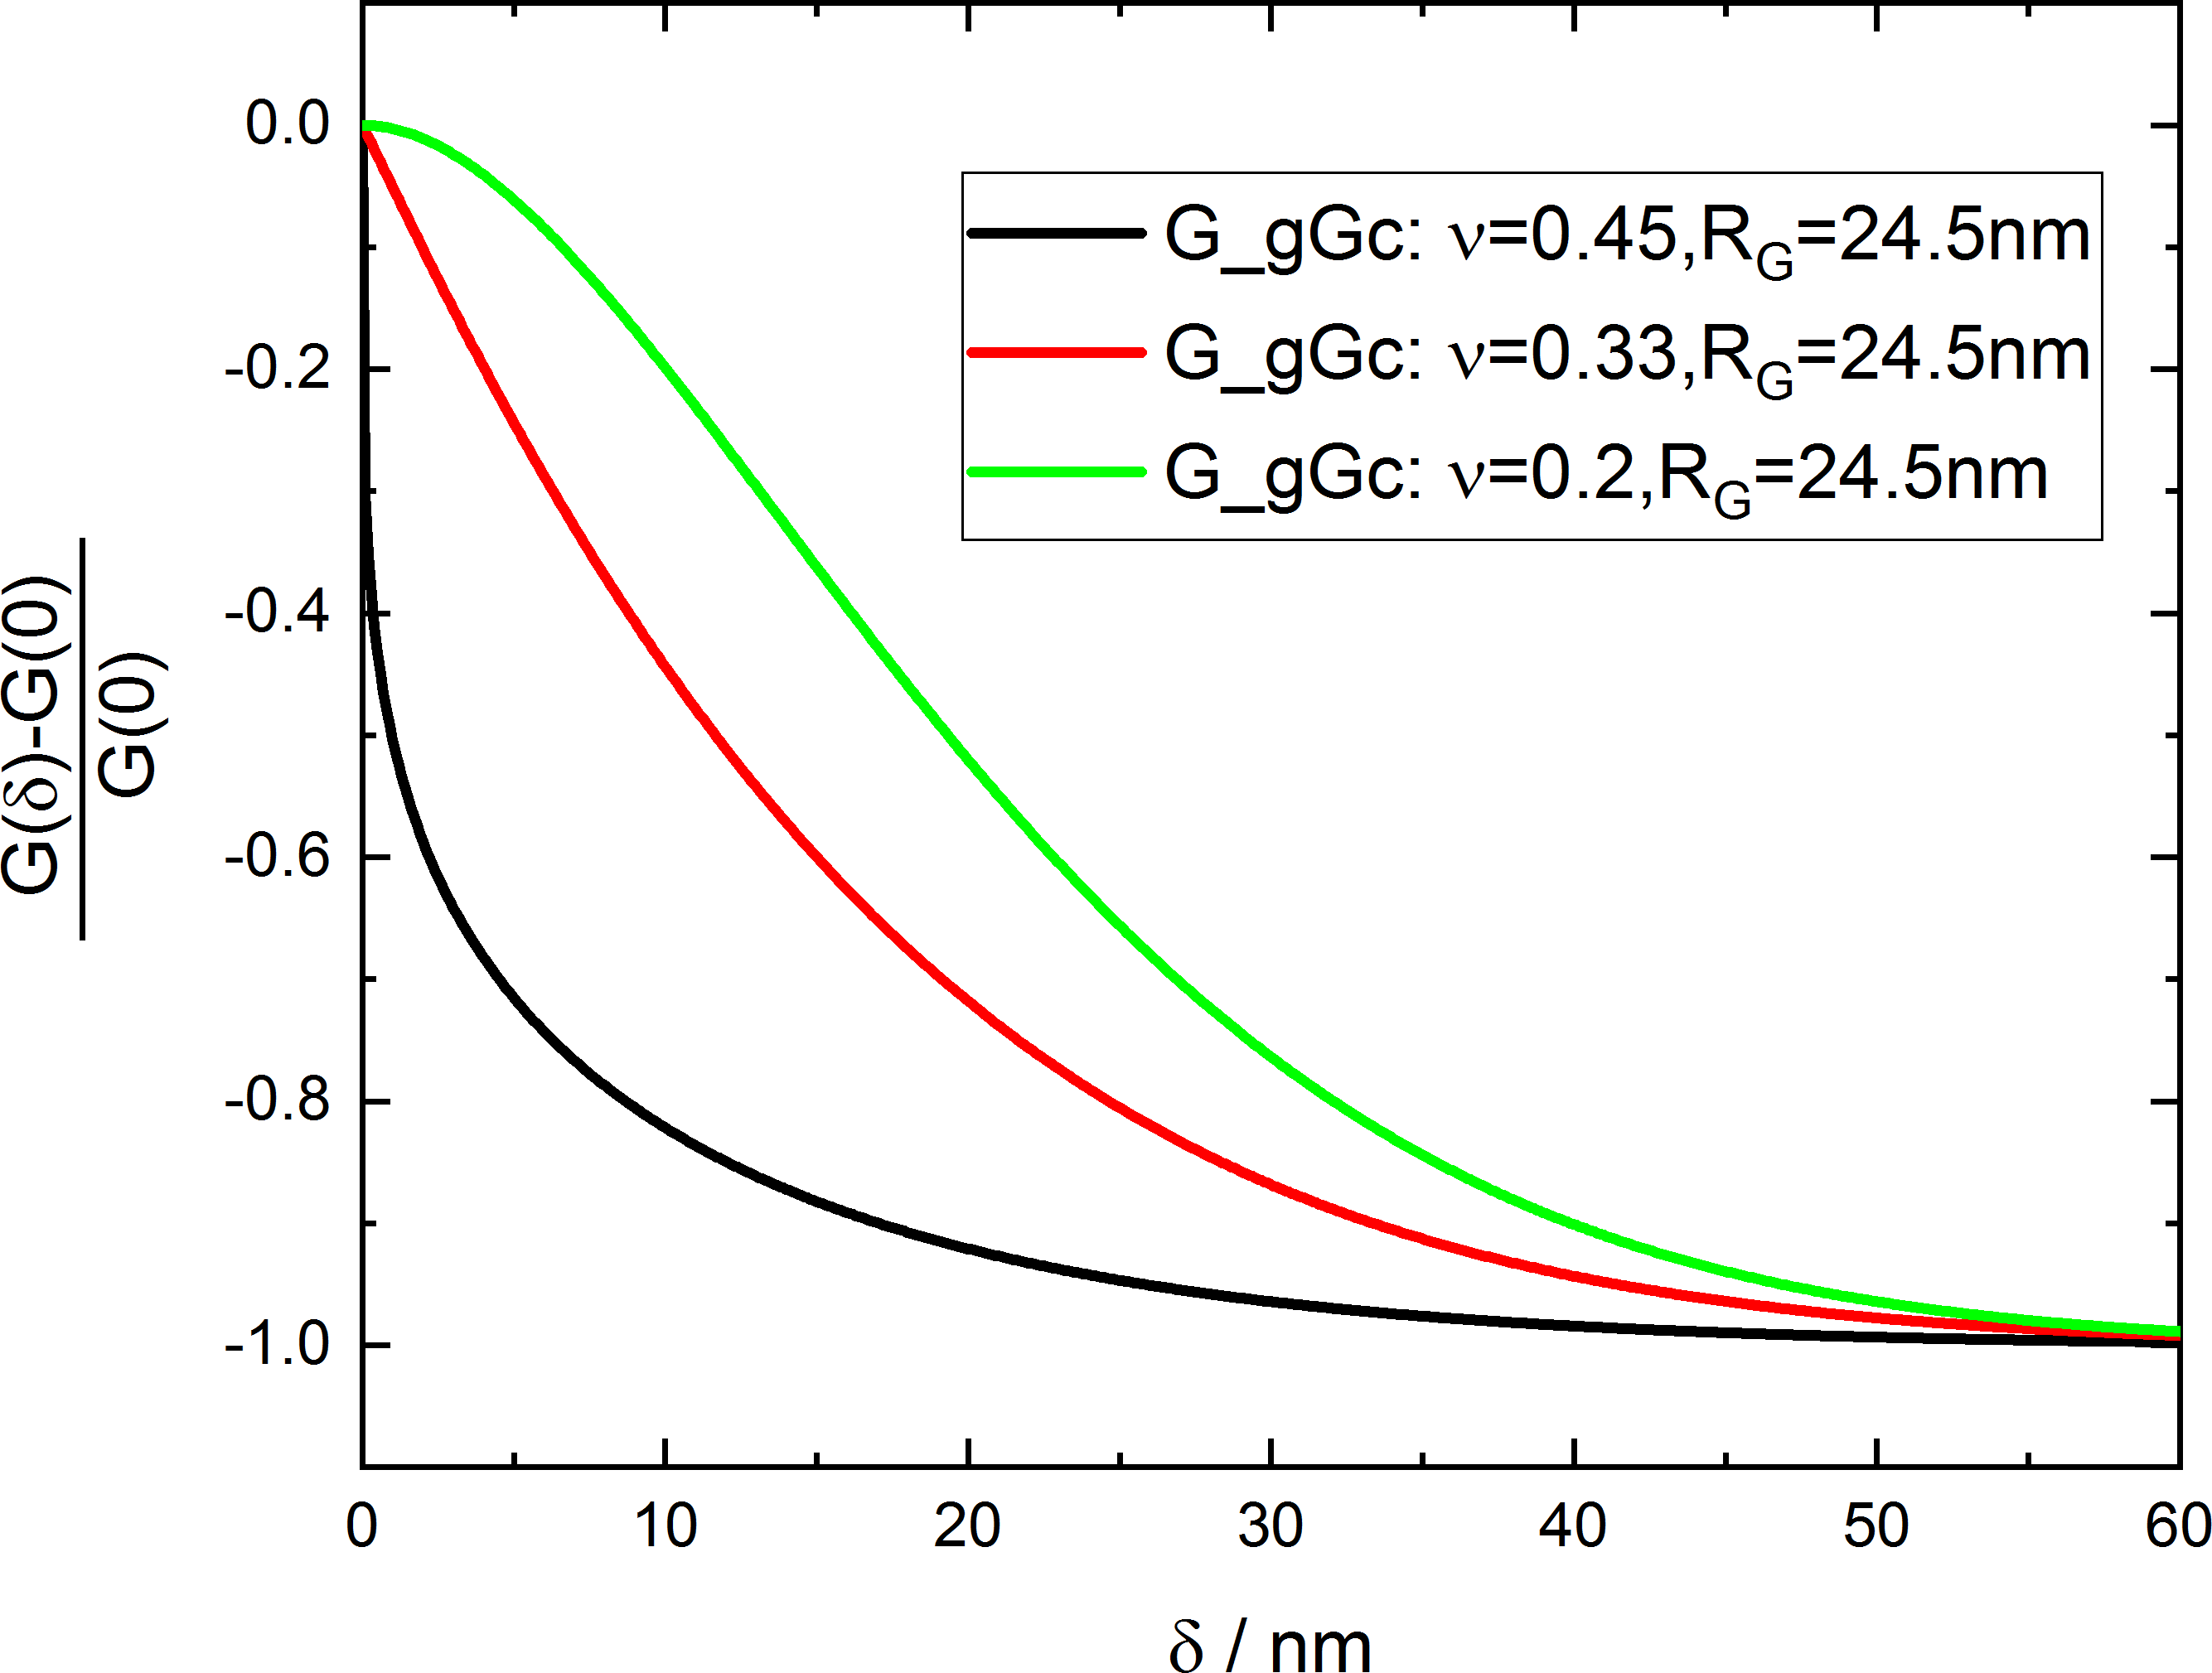
\includegraphics[width=0.7\textwidth]{../images/form_factor/SESANS/G_gGc.png}
\end{center}
\caption{Projected correlation functions of the generalised Gaussian coil model with $R_g=24.5nm$}
\label{fig:G_gDAB}
\end{figure} 